\documentclass[tikz, border=50pt]{standalone}

\usepackage{tikz}
\usepackage{medl_colors}
\usepackage{graphicx}
\usetikzlibrary{shapes.multipart, shapes.geometric, arrows.meta}
\usetikzlibrary{matrix, calc, positioning,fit}
\usepackage{xstring}

\newif\ifmember
\makeatletter
\newcommand{\MemberQ}[2]{\global\memberfalse%
\@for\next:=#1\do{\ifnum\next=#2\global\membertrue\fi}}
\makeatother

\begin{document}
\begin{tikzpicture}

\newcommand\circles[3]
{
    \foreach \i in {1,2,3,4,5,6,7}
    {
    \IfEq{#3}{1}%
        {
            \node [draw=green2, circle, minimum size=.6cm, fill=green0] (circle#1\i) at(#2, -\i+4) {};
        }
        {
            \MemberQ{2,3,6}{\i}
            \ifmember
            {
                \node [draw=green2, circle, minimum size=.6cm] (circle#1\i) at(#2, -\i+4) {};
                \draw[rotate = 45] (circle#1\i.north) -- (circle#1\i.south);
                \draw[rotate = 45] (circle#1\i.west) -- (circle#1\i.east);
            }
            \else%
            {
                \node [draw=green2, circle, minimum size=.6cm, fill=green0] (circle#1\i) at(#2, -\i+4) {};
            }
            \fi
        }
    }
}

\node (rect) at (0,0) [draw,fill=pink1, minimum width=1.5cm,minimum height=2cm] (rectangle)  {C};

\node[trapezium,
    draw = green2,
    fill = green0,
    text = black,
    align=center,
    trapezium angle=80,
    minimum height=3cm,
    shape border rotate=270,
    left of = rectangle, node distance = 4cm ] (t1) { Encoder\\E};  

\node[trapezium,
    draw = blue1,
    fill = blue0,
    text = black,
    align=center,
    trapezium angle=80,
    minimum height=3cm,
    shape border rotate=90,
    right of = rectangle, node distance = 4cm ] (t2) { Decoder\\D};    

\node[left of = t1, node distance = 4cm, draw=green2, fill=green0, minimum width=1cm,minimum height=8cm ] (input) {};

\node[right of = t2, node distance = 4cm, draw=blue1,fill=blue0, minimum width=1cm,minimum height=8cm] (output)  {x\textquotesingle};

\draw [-Triangle] (t1.east) -- (rectangle.west) node[midway,right] {};
\draw [-Triangle] (rectangle.east) -- (t2.west) node[midway,right] {};
\draw [-Triangle] (input.east) -- (t1.west) node[midway,right] {};
\draw [-Triangle] (t2.east) -- (output.west) node[midway,right] {};

\circles{1}{-8}{2};
\circles{2}{-10}{2};
\circles{3}{-12}{1};

\node[scale = .5, below of = circle17, node distance = 4cm] (inputpic1)  {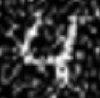
\includegraphics {images/partially_destroyed_input.png}};
\node[scale = .5, below of = circle27, node distance = 4cm] (inputpic2)  {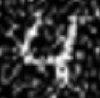
\includegraphics {images/partially_destroyed_input.png}};
\node[scale = .5, below of = circle37, node distance = 4cm] (inputpic3)  {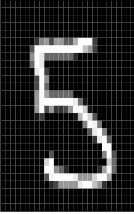
\includegraphics {images/original_input.png}};
\node[scale = .5, below of = output, node distance = 10cm] (outputpic)  {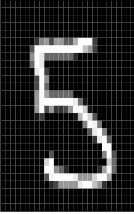
\includegraphics {images/original_input.png}};



\node[above of=rectangle, align=center, node distance=2cm] {Bottleneck!};
\node[above of=circle11, align=center, node distance=2cm] {Input\\$\tilde X$};
\node[above of=circle21, align=center, node distance=2cm] {Partially\\Destroyed\\Input};
\node[above of=circle31, align=center, node distance=2cm] (tinput) {Original\\Input\\X};
\node[above of=output, align=center, node distance=5cm](toutput) {Reconstructed\\Input};

\draw[dashed] ([yshift=1cm]tinput.north) -- ([yshift=1cm]toutput.north) node[midway,anchor=center, fill=white](tcenter) {Ideally they are identical};
\node[below of = tcenter, node distance = .5cm] {$\tilde X \approx X$\textquotesingle};

\draw[dashed,-Triangle] ([yshift=1cm]tinput.north) -- (tinput.north); 
\draw[dashed,-Triangle] ([yshift=1cm]toutput.north) -- (toutput.north); 

\end{tikzpicture}
\end{document}